\label{chap:results}

This chapter will perfom experiments to find out whether or not
\emph{stacked recommenders} is a viable technique.
We will perform three experiments to 
test the three hypotheses outlined in Section 
\ref{sec:hypotheses}.
The next chapter will discuss implications 
and limitations of the results.

\section{Three Experiments}

Table \ref{table:experiments} shows the experiments that will test our technique.
Experiments 1 \emph{\&} 2 will test hypotheses H1 \emph{\&} H2.
We will measure the performance of adaptive recommenders compared to standard and aggregate recommenders.
Experiment 3 will test hypothesis H3.
We will try using our method to personalize sets of search results in a number of ways.
The first two experiments will be quantitative measurements of prediction aggregation performance.
The last experiment will be a qualitative exploration of personalized search with adaptive recommenders.
In particular, we will look at how different prioritizations of the IR model scores influence the final rankings.

\vspace{1em}
\begin{table}[h]
  \begin{tabular*}{\textwidth}{ l l l l l l l }
    \toprule
      ~ & 
      \emph{mission} &
      \emph{hypotheses} &
      \emph{dataset} &
      \emph{users} &
      \emph{items} &
      \emph{ratings} \\
    \midrule
    
    Experiment 1 &
    pred.agg. &
    H1, H2 &
    MovieLens &
    943 &
    1,682 &
    100,000 \\
    
    Experiment 2 &
    pred.agg. &
    H1, H2 &
    Jester &
    24,983 &
    100 &
    1,832,275 \\

    Experiment 3 &
    rank.agg. &
    H3 &
    MovieLens &
    6,040 &
    3,900 &
    1,000,000 \\
    
    \bottomrule 
  \end{tabular*}
  \caption[List of Experiments]{List of Experiments performed in this chapter.}
  \label{table:experiments}
\end{table}

\noindent
As seen in Table \ref{table:experiments}, 
we will use two distinct datasets in the experiments.
Each dataset have different numbers of items, users and ratings.
This is a desirable property.
Testing adaptive recommenders in different scenarios
will help us achieve more reliable results.

First is the MovieLens dataset\footnote{
See http://www.grouplens.org/node/73 --- accessed 10.05.2011}.
This dataset is often used to test the performance of recommender systems
(as described in 
\citet[p.9]{Alshamri2008}, \citet[p.4]{Lemire2005}, \citet[p.1]{Adomavicius2005} and \citet[p.2]{Herlocker2004}).
It consists of a set of users, a set of movies, and a set of movie ratings from users,
on the scale $1$ through $5$.
We chose two subsets of the entire MovieLens collection.
For Experiment 1 we use a subset of 100,000 ratings from 943 users on 1,682 movies.
For Experiment 3 we use a much larger subset in order to
have more items available for the IR model.
This subset has 1,000,000 ratings from 6,040 users of 3,900 movies.

The MovieLens dataset also comes with meta-data on users, such as
gender, age and occupation. There is also meta-data on movies,
such as its title, release date and genre. 
In Experiment 1, we are only interested in the ratings matrix of this dataset.
The titles of movies will be used in Experiment 3.

Our second set of ratings comes from the Jester dataset\footnote{
See \url{eigentaste.berkeley.edu/dataset/} ---
accessed 22.05.2011}.
This is a set of 100 \emph{jokes} rated by users on a continuous scale.
As with MovieLens, this dataset is also commonly used
to test recommender systems (as described in
\cite{Goldberg2001}, \citet[p.14]{Herlocker2004}, \citet[p.5]{Adomavicius2005} and \citet[p.30]{Ahn2004}).
This dataset has many more users than those used in the other experiments.
On the other hand, there are significantly fewer items than in the other dataset.
The widely varying number of items, users and ratings in our selected datasets
will give us more dimensions along which to verify our results.

Jester also has ratings on a different scale than the MovieLens dataset.
While the movies are rated on a discrete scale from $1$ through $5$,
the items in Jester are rated on a continuous scale from $-10$ to $10$.
However, in order to easily compare the measurements on both datasets,
the ratings in Jester were converted to be on the scale $1-5$.
Still, the difference between ordinal and continuous ratings remains,
and will give us another differing quality to verify our results.

In another effort to achieve reliable results, 
both datasets were split into multiple disjoint subsets.
We need disjoint subsets in order to perform cross-validation testing.
This entails running the same experiments across all subsets and averaging the results.
Each dataset is split into five sets which are again split into training and testing sets:

\begin{eqsp}
  D_n = \{ d_1 = \{base_1, test_1\}, d_2 = \{base_2, test_2\}, ..., d_5 = \{base_5, test_5\} \}
\end{eqsp}

The $base_x$ and $test_x$ pairs are disjoint 80\% / 20\% splits of the data in the subsets.
We shall perform five-fold cross-validation across all these sets in our experiments.
This way we can be more certain that our results are reliable,
and not because of local effect in parts of the data.
As previously explained, the $base$ sets are further split using bootstrap aggregation,
into random subsets for training the standard recommender models.
The entire base set is then used to train the adaptive error estimating recommenders.
The corresponding $test$ sets will be used to evaluate our performance on the subsets.

Before performing our experiments,
let us take a closer look at the different types of recommender systems we will use.

\section{Recommenders}

In addition to the dataset, we need a number of recommender systems
that can predict unknown ratings between users and items.
As we have seen, standard recommenders will be used for both the basic predictions,
and for the accuracy estimations for each basic prediction.

Naturally, we need a number of different recommenders, preferably ones that consider
disjoint patterns in the data. Table \ref{table:results:methods}
gives a short overview of the recommender systems we shall employ.
See Section \ref{sec:recommender} for more information on the different
types of recommenders, and Appendix \ref{appendix:implementation}
for information on how these were implemented in the following experiments.

\subsection{Basic Recommenders}

\begin{table}[t]
  \begin{tabular*}{\textwidth}{ l l l l }
    \toprule
    ~ & \emph{method} &  \emph{algorithm} & \emph{description} \\
    \midrule
    S & svd1          & SVD                   & ALSWR factorizer, 10 features. \\
    S & svd2          & SVD                   & ALSWR factorizer, 20 features. \\
    S & svd3          & SVD                   & EM factorizer, 10 features. \\
    S & svd4          & SVD                   & EM factorizer, 20 features. \\
    S & slope\_one    & Slope One             & Rating delta computations. \\
    S & item\_avg     & Baseline              & Based on item averages. \\ 
    S & baseline      & Baseline              & Basd on user and item averages.\\ 
    S & cosine   	    & Cosine similarity     & Weigted ratings from similar items.\\ 
    S & knn       	  & Pearson Corr.         & Weighted ratings from similar users.\\
    \midrule
    A & median    	  & Aggregation           & Median rating from the above methods. \\
    A & average    	  & Aggregation           & Average rating from the above methods. \\
    A & stacked       & Adaptive agg.         & Accuracy predictions from error models. \\
    \bottomrule
  \end{tabular*}
  \caption[Stacked Modeling Methods]{
    Stacked modeling methods: A short description of each of the recommender methods
    used in our experiment. See Section \ref{sec:recommender} for more information.
    For the SVD methods, the factorizers refers to algoriithms used to factorize the ratings matrix.
    An EM factorizer uses the Expectation-Maximization algorithm to find the factors.
    An ALSWR factorizer performs the same factorization with a least-squares approach \citep{Zhou2008}.
    The number of features refers to the truncation of the factors in order to reduce the taste-space.
  }
  \label{table:results:methods}
\end{table}

As seen in Table \ref{table:results:methods}, we have two types of recommenders:
First, we have the basic recommenders, denoted by \emph{S} in the table.
These recommenders each look at the data in different ways to arrive at predicted ratings.
We chose this wide range of recommenders for just this reason:
as previously explained, the performance of aggregate recommenders
are more dependent on the disimilarity of the basic recommenders
than their individual performance.

Let us briefly explain how each basic recommender works.
The SVD methods look for global patterns in the data 
by reducing the ratings-space into a concept-space.
By reducing this space, the algorithm is able to find
latent relations, such as groups of movies that has the same
rating pattern, or groups of users that often rate in a similar manner.

The Slope One and baseline algorithms look at average
ratings for items and from users, and use these to predict ratings.
The cosine similarity algorithm looks for items that are rated
similarly by the same users, and infers item similarity from this measure.
New ratings are then predicted by taking known ratings of other items,
weighted by their item's similarity to the new item.

The KNN algorithm employs yet another approach. This algorithm,
similar in strategy to the cosine similarity algorithm,
looks for users with similar rating patterns.
The similarity is measured with the Pearson Correlation Coefficient.
Predictions are created by collecting ratings from similar users
of the item in question, weighted by their respective similarity.
See Section \ref{sec:recommender} for more 
detailed information on how these recommenders work. 

\subsection{Stacked Recommenders}

The second type of recommenders are the aggregation methods, 
that combine the result of each of the basic recommender systems.
In addition to our stacked recommender method
(denoted with the key \emph{stacked} in Table \ref{table:results:methods}),
we have the median- and average-based aggregators.
The median aggregator choses the median value of the predictions
produced by the standard recommenders.
Similarly, the average aggregator takes the mean of the
standard predictions.
While not complex in nature, these methods
will help us see how our method compares to simple, traditional
aggregation techniques.

As explained in Section \ref{sec:usermetamodeling},
any basic recommender system can be used for the stacked method.
The only difference is how this method is trained:
while the basic methods are trained using the ratings matrix,
the stacked methods are trained using the error model,
as seen in Listing \ref{code:training}.
In other words, we have as many possibilities for choosing
the stacked recommenders as the basic recommenders.

For our experiment, we went with SVD recommenders
for each of the stacked models.
That is, each basic recommender method gets a secondary 
accuracy predicting recommender, which in this case is a 
standard SVD recommender.
The SVD recommender is a natural choice in this case,
since we wish to uncover latent patterns of accuracy
for each model.
Examples of these patterns include groups of items
or users a specific recommender works well for.

The choices of recommenders will be further discussed
in Chapter \ref{chap:discussion}.
For now, let us see how we determined the performance of each method.




\section{Evaluation Strategies}

To evaluate how our model performs, we need a measure
for computing the total error across a large number of predictions.
The canonical measure for estimating the error of a 
predictions from a recommender system
is the \emph{Root mean squared error} (RMSE) measure
(e.g. \citet[p17]{Herlocker2004}, \citet[p13]{Adomavicius2005} and \citet[p6]{Bell2007}).
We shall use this measure to estimate the performance
of our adaptive prediction aggregation algorithms.
The RMSE of a set of estimations $\hat{R}$, 
compared to a set of known ratings $R$, is defined as

\begin{eqsp}
  \mathrm{RMSE}(\hat{R},R) = \sqrt{\mathrm{E}((\hat{R} - R)^2)}
  = \sqrt{\frac{
      \sum_{i=1}^{n} (\hat{R}_i - R_i)^2
    }{
      n
    }},
\end{eqsp}
%
where $n$ is the total number of predictions.
The RMSE combines a set of errors into one single combined error.
A beneficial feature of the RMSE is that the resulting error 
will be on the same scale as the estimations. In other words,
if we are predicting values on the scale $1-5$, the computed error
will be on this scale as well. In this case, an error of $1$
would then say that we are on average $1$ point away from the true 
ratings on our $1-5$ scale.

RMSE is a non-linear error estimator.
This means that larger errors are harsly punished.
Because the differences are squared by the formula,
many small errors are much less significant than a few big errors.
In other words, the RMSE will judge methods that provide
stable predictions more favorably
than methods that, while precise, have a few items
or users for which the method breaks down.
For example, when the RMSE was used in the Netflix movie recommendation
competition \cite{Linden2009}, the participating teams
found that a few hard to predict movies often 
single-handedly corrupted the total error measure.

While the RMSE works well for evaluating scalar predictions,
we need another measure for considering a predicted sorting 
from rank estimation methods.
Here, we are not interested in the predicted scores,
but rather in which position each item appears in a sorted list of results.
This is for instance needed when measuring the performance of a
personalized search engine.
Because of this, we are interested in examining how 
personalization with stacked recommenders affects the rankings
from an IR method.

To answer our three hypotheses, we have performed two experiments.
The first experiment evaluates our method when used for
adaptive prediction aggregation, comparing it to 
the methods given in Table \ref{table:results:methods}.
This will help us answer hypotheses H1 and H2.
The second experiment will evaluate our performance
in adaptive rank aggregation, in order to answer hypothesis H3.
For more information on how the algorithms
in this experiment were implemented, see Appendix \ref{appendix:implementation}.




\section{Prediction Aggregation}

\begin{table}[p]
  \centering

  \textbf{Results from Experiment 1}

  \vspace{3em}

  \begin{tabular*}{\textwidth}{ l p{3cm} p{1.5cm} p{1.5cm} p{1.5cm} p{1.5cm} p{1.5cm} }
    \toprule
      ~ & \emph{method} & 
      $d_1$ & $d_2$ & $d_3$ & $d_4$ & $d_5$ \\ 
    \midrule
    S & svd1          & 1.2389	  & 1.1260	  & 1.1327	  & 1.1045	  & 1.1184	 \\
    S & svd2          & 1.2630	  & 1.1416    & 1.1260	  & 1.1458	  & 1.1260	 \\
    S & svd3          & 1.0061	  & 0.9825	  & 0.9830	  & 0.9815	  & 0.9797	 \\
    S & svd4          & 1.0040	  & 0.9830	  & 0.9849	  & 0.9850	  & 0.9798	 \\
    S & slope\_one    & 1.1919	  & 1.0540	  & 1.0476	  & 1.0454	  & 1.0393   \\
    S & item\_avg     & 1.0713	  & 0.9692	  & 0.9662	  & 0.9683	  & 0.9725	 \\
    S & baseline       & 1.0698	  & 0.9557	  & 0.9527	  & 0.9415	  & 0.9492	 \\
    S & cosine   	    & 1.1101	  & 0.9463	  & 0.9412	  & 0.9413	  & 0.9382	 \\
    S & pcc       	  & 1.4850	  & 1.1435	  & 1.1872    & 1.2156	  & 1.2022	 \\
    \midrule                                                                    
    A & median    	  & 0.9869	  & 0.8886	  & 0.8857    & 0.8857	  & 0.8855	 \\
    A & average    	  & 0.9900	  & 0.8536	  & 0.8525	  & 0.8525	  & 0.8519	 \\
    A & adaptive       & \textbf{0.9324}	  & \textbf{0.8015}	  & \textbf{0.7993}  & \textbf{0.8238} & \textbf{0.8192} \\
    \bottomrule
  \end{tabular*}

  \vspace{3em}

  \begin{tabular*}{\textwidth}{ l p{3cm} p{2cm} p{2cm} p{2cm} p{2cm} }
    \toprule
      ~ & \emph{method} & 
      \emph{min} & \emph{max} & \emph{mean} & $\sigma$\\
    \midrule
    S & svd1          & 1.1045	& 1.2389	& 1.1441	& 0.2197 \\
    S & svd2          & 1.1260	& 1.2630	& 1.1605	& 0.2277 \\
    S & svd3          & 0.9797	& 1.0061	& 0.9865	& 0.0991 \\
    S & svd4          & 0.9798	& 1.0040	& 0.9873	& \textbf{0.0924} \\
    S & slope\_one    & 1.0393	& 1.1919	& 1.0756	& 0.2415 \\
    S & item\_avg     & 0.9662	& 1.0713	& 0.9895	& 0.2023 \\
    S & baseline       & 0.9415	& 1.0698	& 0.9738	& 0.2196 \\
    S & cosine   	    & 0.9382	& 1.1101	& 0.9754	& 0.2595 \\
    S & pcc       	  & 1.1435	& 1.4850	& 1.2467	& 0.3487 \\
    \midrule            
    A & median    	  & 0.8855	& 0.9865	& 0.9065	& 0.2005 \\
    A & average    	  & 0.8519	& 0.9900	& 0.8801	& 0.2344 \\
    A & adaptive       & \textbf{0.7993}	& \textbf{0.9324}	& \textbf{0.8352}	& 0.2225 \\
    \bottomrule
  \end{tabular*}
  \vspace{2em}

  \caption[Results from Experiment 1]{
    Results from experiment 1 (MovieLens):
    Each cell gives an RMSE value, on the scale 1-5.
    The first table gives errors for each subset of the data ($d_x$).
    Lower values indicate better results.
    Bold values indicate the best result in each column.
    S refers to singular methods, and A to aggregation methods.
    $\sigma$ refers to the standard deviation of each method across the subsets.
  }
  \label{table:results:e1}
\end{table}



done: 4,5

  Results
  ----------------------------------------------------------------------------------------------------
  svd1         	  4: 1.08168	  5: 1.09346	min: 1.08168	max: 1.09346	avg: 1.08757	stddev: 0.076746
  svd3         	  4: 0.9479	    5: 0.94826	min: 0.9479	  max: 0.94826	avg: 0.94808	stddev: 0.013416
  svd4         	  4: 0.94892	  5: 0.9459	  min: 0.9459	  max: 0.94892	avg: 0.94741	stddev: 0.038859
  knn3         	  4: 1.02418	  5: 1.0243	  min: 1.02418	max: 1.0243	  avg: 1.02424	stddev: 0.007746
  knn4         	  4: 1.02304	  5: 1.0244	  min: 1.02304	max: 1.0244	  avg: 1.02372	stddev: 0.026077
  slope_one    	  4: 1.11074	  5: 1.11703	min: 1.11074	max: 1.11703	avg: 1.113885	stddev: 0.05608
  baseline     	  4: 1.10294	  5: 1.10662	min: 1.10294	max: 1.10662	avg: 1.10478	stddev: 0.042895
  cosine       	  4: 1.08539	  5: 1.07813	min: 1.07813	max: 1.08539	avg: 1.08176	stddev: 0.060249
  m_average    	  4: 0.91857	  5: 0.91733	min: 0.91733	max: 0.91857	avg: 0.91795	stddev: 0.0249
  m_median     	  4: 0.92481	  5: 0.9225	  min: 0.9225	  max: 0.92481	avg: 0.923655	stddev: 0.033985
  svd2         	  4: 1.08591	  5: 1.08837	min: 1.08591	max: 1.08837	avg: 1.08714	stddev: 0.035071
  knn1         	  4: 1.18459	  5: 1.1921	  min: 1.18459	max: 1.1921	  avg: 1.188345	stddev: 0.061278
  knn2         	  4: 1.16415	  5: 1.18468	min: 1.16415	max: 1.18468	avg: 1.174415	stddev: 0.101316
  m_svd        	  4: 0.96698	  5: 0.79647	min: 0.79647	max: 0.96698	avg: 0.881725	stddev: 0.291985

  avgs:
  [[:m_svd, 0.881725],
   [:m_average, 0.91795],
   [:m_median, 0.923655],
   [:svd4, 0.94741],
   [:svd3, 0.94808],
   [:knn4, 1.02372],
   [:knn3, 1.02424],
   [:cosine, 1.08176],
   [:svd2, 1.08714],
   [:svd1, 1.08757],
   [:baseline, 1.10478],
   [:slope_one, 1.113885],
   [:knn2, 1.174415],
   [:knn1, 1.188345]]



done 1:

  Results
  ----------------------------------------------------------------------------------------------------
  svd1           	  1: 1.08626	min: 1.08626	max: 1.08626	avg: 1.08626	stddev: 0.0
  svd2           	  1: 1.08119	min: 1.08119	max: 1.08119	avg: 1.08119	stddev: 0.0
  svd3           	  1: 0.94702	min: 0.94702	max: 0.94702	avg: 0.94702	stddev: 0.0
  svd4           	  1: 0.95061	min: 0.95061	max: 0.95061	avg: 0.95061	stddev: 0.0
  knn3           	  1: 1.02663	min: 1.02663	max: 1.02663	avg: 1.02663	stddev: 0.0
  knn4           	  1: 1.02323	min: 1.02323	max: 1.02323	avg: 1.02323	stddev: 0.0
  slope_one      	  1: 1.11015	min: 1.11015	max: 1.11015	avg: 1.11015	stddev: 0.0
  cosine         	  1: 1.07766	min: 1.07766	max: 1.07766	avg: 1.07766	stddev: 0.0
  m_average      	  1: 0.91888	min: 0.91888	max: 0.91888	avg: 0.91888	stddev: 0.0
  m_median       	  1: 0.92529	min: 0.92529	max: 0.92529	avg: 0.92529	stddev: 0.0
  knn2           	  1: 1.1896	min: 1.1896	max: 1.1896	avg: 1.1896	stddev: 0.0
  baseline       	  1: 1.09193	min: 1.09193	max: 1.09193	avg: 1.09193	stddev: 0.0
  knn1           	  1: 1.1808	min: 1.1808	max: 1.1808	avg: 1.1808	stddev: 0.0
  m_svd          	  1: 0.93866	min: 0.93866	max: 0.93866	avg: 0.93866	stddev: 0.0

  avgs:
  [[:m_average, 0.91888],
   [:m_median, 0.92529],
   [:m_svd, 0.93866],
   [:svd3, 0.94702],
   [:svd4, 0.95061],
   [:knn4, 1.02323],
   [:knn3, 1.02663],
   [:cosine, 1.07766],
   [:svd2, 1.08119],
   [:svd1, 1.08626],
   [:baseline, 1.09193],
   [:slope_one, 1.11015],
   [:knn1, 1.1808],
   [:knn2, 1.1896]]



Our first hypothesis, H1, states that:
{
  \itshape
  the accuracy of relevance predictions can be improved
  through adaptive recommender aggregation.
}
The second hypothesis, H2, states:
{
  \itshape
  adaptive aggregation can achieve higher accuracy than global and generalized aggregation methods.
}

In order to verify these hypotheses, we performed adaptive prediction aggregation
through stacked recommenders on the five datasets described in the previous section.
Table \ref{table:results:e1} gives the results from this experiment.
Each cell corresponds to the RMSE values for each dataset,
for each recommender and aggregation approach.
The bottom entry in this table refers to our stacked recommenders method.
As seen in this table, the stacked recommender achieved
lower RMSE values than any of the other applied methods.

Statistics from the results in Table \ref{table:results:e1} 
are given in Table \ref{table:results:e1:sum}.
These values are the minimum, maximum and mean values
for each of the methods. We also include
the standard deviation ($\sigma$) for each method,
across our datasets.
This table confirms the results from the full results table:
Our stacked recommenders approach improves the mean performance
of our system.
The mean performance, along with the standard deviation
are shown in Figure \ref{plot:rmse}.

%\begin{figure*}[!t]
\center

\pgfplotsset{width=\textwidth,height=8cm}
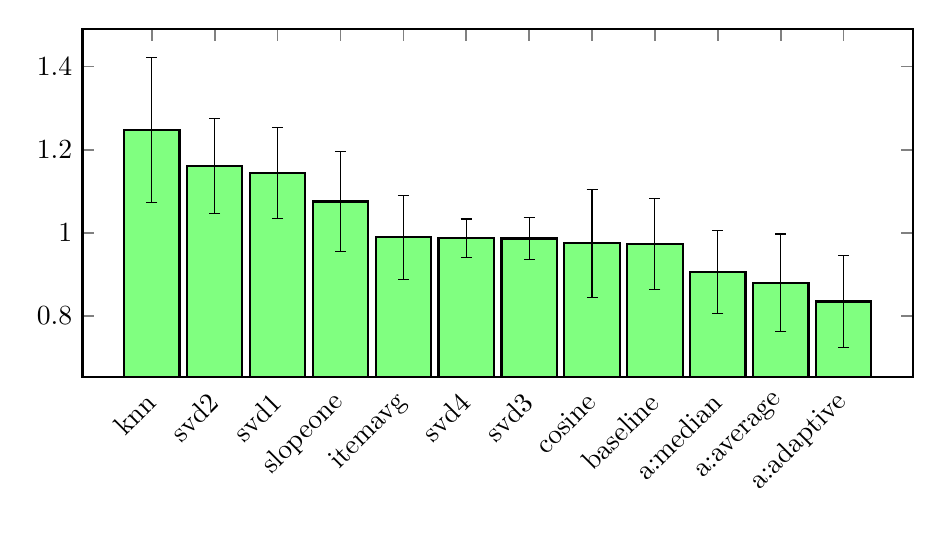
\begin{tikzpicture}

\begin{axis}[
      symbolic x coords={
        knn,svd2,svd1,slopeone,itemavg,svd4,svd3,cosine,baseline,a:median,a:average,a:adaptive},
      xtick=data,
      x tick label style={rotate=45,anchor=east,yshift=-0.5em,xshift=-0.2em},
      bar width=20pt
    ]

    \addplot [ybar,fill=green!50,error bars/.cd,y dir=both,y explicit] coordinates {
      (knn, 1.2467) +- (0,0.17435) 
      (svd2, 1.1605) +- (0,0.11385)
      (svd1, 1.1441) +- (0,0.10985)
      (slopeone, 1.0756) +- (0,0.12075)
      (itemavg, 0.9895) +- (0,0.10115)
      (svd4, 0.9873) +- (0,0.0462)
      (svd3, 0.9865) +- (0,0.04955)
      (cosine, 0.9754) +- (0,0.12975)
      (baseline, 0.9738) +- (0,0.1098)
    %};
    %\addplot [ybar,fill=blue!50] coordinates {
      (a:median, 0.9065) +- (0,0.10025)
      (a:average, 0.8801) +- (0,0.1172)
      (a:adaptive, 0.8352) +- (0,0.11125)
    };
\end{axis}

\end{tikzpicture}
\vspace{-1em}
\caption[Average RMSE Plot]{
  Average RMSE plot: This plot shows the average RMSE for each method, and each aggregation method (denoted "a:").
  The actual numbers are given in Table \ref{table:results:e1}.
  The error bars indicate the standard deviation of each method.
  Note the scale on the y-axis --- the errors are not as pronounced as they might seem. 
}
\label{plot:movielens}
\end{figure*}




\begin{figure}[p]
  \centering
  \subfloat[Experiment 1]{\label{fig:rmse:e1}
\pgfplotsset{width=\textwidth,height=8cm}
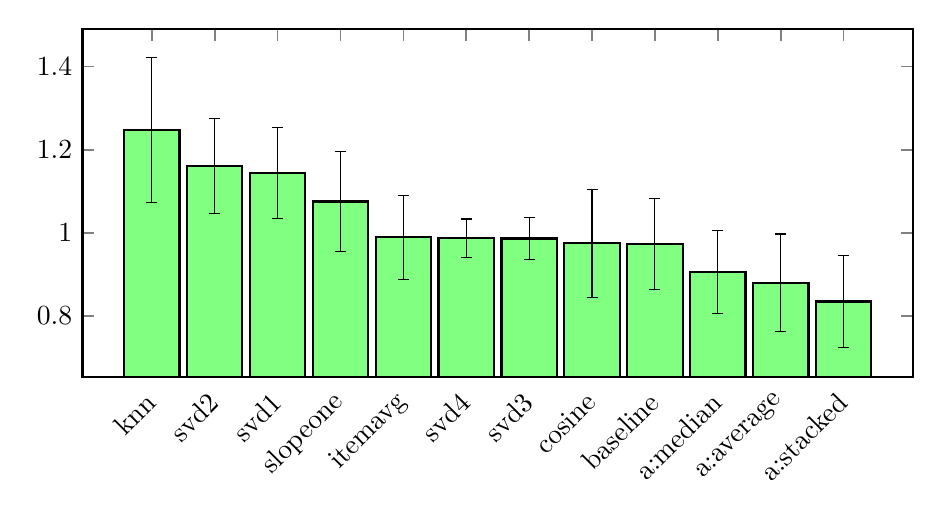
\begin{tikzpicture}
\begin{axis}[
      symbolic x coords={
        knn,svd2,svd1,slopeone,itemavg,svd4,svd3,cosine,baseline,a:median,a:average,a:stacked},
      xtick=data,
      x tick label style={rotate=45,anchor=east,yshift=-0.5em,xshift=-0.2em},
      bar width=20pt
    ]
    \addplot [ybar,fill=green!50,error bars/.cd,y dir=both,y explicit] coordinates {
      (knn, 1.2467) +- (0,0.17435) 
      (svd2, 1.1605) +- (0,0.11385)
      (svd1, 1.1441) +- (0,0.10985)
      (slopeone, 1.0756) +- (0,0.12075)
      (itemavg, 0.9895) +- (0,0.10115)
      (svd4, 0.9873) +- (0,0.0462)
      (svd3, 0.9865) +- (0,0.04955)
      (cosine, 0.9754) +- (0,0.12975)
      (baseline, 0.9738) +- (0,0.1098)
    %};
    %\addplot [ybar,fill=blue!50] coordinates {
      (a:median, 0.9065) +- (0,0.10025)
      (a:average, 0.8801) +- (0,0.1172)
      (a:stacked, 0.8352) +- (0,0.11125)
    };
\end{axis}
\end{tikzpicture}}

\vspace{1em}
 
  \subfloat[Experiment 2]{\label{fig:rmse:e2}
\pgfplotsset{width=\textwidth,height=8cm}
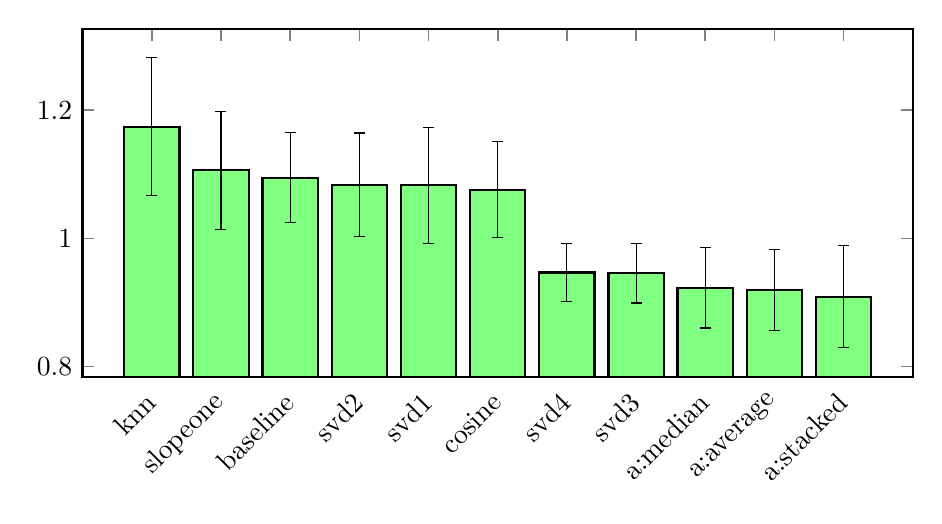
\begin{tikzpicture}
\begin{axis}[
      symbolic x coords={
        knn,slopeone,baseline,svd2,svd1,cosine,svd4,svd3,a:median,a:average,a:stacked},
      xtick=data,
      x tick label style={rotate=45,anchor=east,yshift=-0.5em,xshift=-0.2em},
      bar width=20pt
    ]
    \addplot [ybar,fill=green!50,error bars/.cd,y dir=both,y explicit] coordinates {
      (knn, 1.1740) +- (0,0.1077) 
      (slopeone, 1.1062) +- (0,0.0918)
      (baseline, 1.0945) +- (0,0.0700)
      (svd2, 1.0835) +- (0,0.0808)
      (svd1, 1.0829) +- (0,0.0905)
      (cosine, 1.0760) +- (0,0.0749)
      (svd4, 0.9467) +- (0,0.0446)
      (svd3, 0.9455) +- (0,0.0464)
    %};
    %\addplot [ybar,fill=blue!50] coordinates {
      (a:median, 0.9227) +- (0,0.0626)
      (a:average, 0.9193) +- (0,0.0630)
      (a:stacked, 0.9091) +- (0,0.0797)
    };
\end{axis}
\end{tikzpicture}}

\vspace{1em}

  \caption[Plots of Results for Experiments 1 \emph{\&} 2]{
    Plots of the average RMSEs for Experiments 1 \emph{\&} 2.
    The actual numbers are given in Tables \ref{table:results:e1}
    \emph{\&} \ref{table:results:e2}.
  }
  \label{plot:rmse}
\end{figure}




\begin{figure}
\center
\tiny

\pgfplotsset{width=\textwidth,height=6cm}
\pgfplotsset{every axis/.append style={
thick,
tick style={semithick}}}

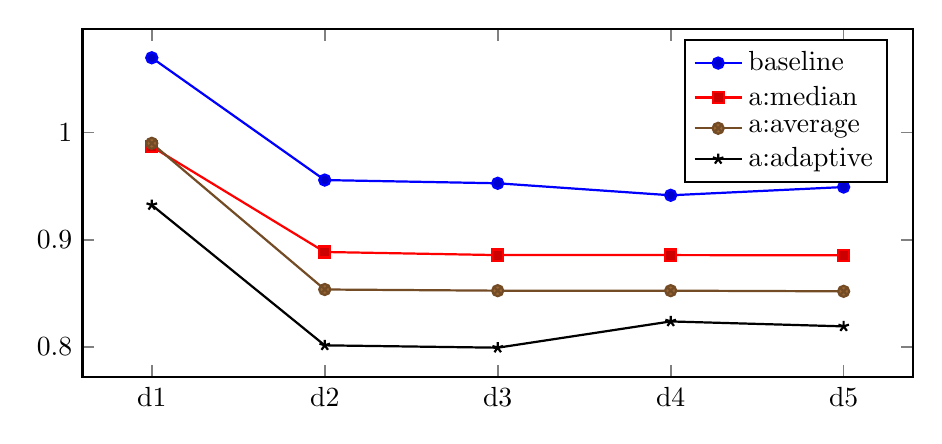
\begin{tikzpicture}

\begin{axis}[
  stack plots=false,
  enlarge x limits=true,
  symbolic x coords={d1,d2,d3,d4,d5},
  xtick=data,
  legend style={
    cells={anchor=west},
    legend pos=north east,
  }
]

\addplot coordinates {
(d1, 1.0698)
(d2, 0.9557)
(d3, 0.9527)
(d4, 0.9415)
(d5, 0.9492)
};
\addlegendentry{baseline}


\addplot coordinates {
(d1, 0.9869)
(d2, 0.8886)
(d3, 0.8857)
(d4, 0.8857)
(d5, 0.8855)
};
\addlegendentry{a:median}
 
\addplot coordinates {
(d1, 0.9900)
(d2, 0.8536)
(d3, 0.8525)
(d4, 0.8525)
(d5, 0.8519)
};
\addlegendentry{a:average}
 
\addplot coordinates {
(d1, 0.9324)
(d2, 0.8015)
(d3, 0.7993)
(d4, 0.8238)
(d5, 0.8192)
};
\addlegendentry{a:adaptive}

\end{axis}
\end{tikzpicture}

\tiny
\caption{
  RMSE Standard deviation caused by dataset $d_1$.
}
\label{plot:datasets}
\end{figure}


Let us take a look at the standard deviation measures from the different methods.
As seen in Figure \ref{plot:rmse}, 
most of the methods, including the stacked models,
exhibit quite a lot of variation in their results.
If these variations occured as a result of unstable
predictions of the same dataset, this would be a substantial problem,
resulting in unreliable predictions.
However, as seen in Figure \ref{plot:datasets},
the standard deviation is mostly caused by the differing
performance across the varying datasets.
As we see, the performance of each of the aggregation methods,
as well as the best performing standard recommender,
follow each other closely. At the same time,
performance varies across the different datasets,
which results in high values for $\sigma$.

What does this mean for hypotheses H1 and H2?
Expressed in terms of this experiment,
H1 posits that stacked recommenders should outperform each of the standard modeling methods
in Table \ref{table:results:e1}.
The adaptive methods blend the results of multiple predictors by estimating the accuracy
on a per-item and per-user basis, satisfying the formulation of H1.

By outperform we mean that our model should have a lower
mean RMSE score than the other singular methods. As we can see in Table \ref{table:results:e1:sum},
\emph{H1 is confirmed for these methods and this dataset}.
While we can not generalize too much on this basis, 
the fact that this dataset is a common testing ground for recommender systems,
that RMSE is the de facto measure for determining performance,
and because of our 5-fold cross-validation, the results allow us 
to confirm hypothesis H1 in these conditions, and likely for other, similar scenarios.
We shall discuss this in Chapter \ref{chap:discussion}.

Similarly, expressed in the same terms, H2 posits that 
our stacked recommenders should outperform the aggregation approaches
given in Table \ref{table:results:e1}.
The \emph{median} and \emph{average} aggregation methods
serve as globalized and generalized aggragation methods,
Stacked recommenders are adaptive in that each prediction is 
aggregated based on the current user and item,
satisfying the language of H2.

As we can see in Table \ref{table:results:e1:sum},
\emph{H2 is confirmed for these methods and this dataset}.
However, as our collection of aggregation methods is a lot simpler
than our collection of recommender systems, the strength of this combination
is notably weaker than that of H1.
Still, the fact that a stacked recommender outperforms these simple aggregation
approaches is a positive result warranting further experiments.
This will also be discussed in Chapter \ref{chap:discussion}.

It would seem then that, based on our experiments, available data
and assumptions of evaluation measures, both H1 and H2 are confirmed.
Our adaptive aggregation approach outperforms both standard recommender
methods and simple generalized aggregation methods.
Notably, our approach is more complex than the methods it outperforms,
so the question whether the methods performance is worth its extra complexity becomes important.
We shall discuss this, and other implications of these results in the next chapter.
For now, let us proceed to the second experiment and hypothesis H3.

\clearpage

\section{Adaptive Rank Aggregation}

While the previous experiment was a quantitative exploration of RMSE values,
this experiment will focus on qualitative traits of rank aggregation.


Test H3

\begin{table}[t]
  \centering 

  \begin{tabular*}{0.9\textwidth}{ r l p{8cm} }
    \multicolumn{3}{l}{Results and their IR ranking score for the query \emph{"new york" or washington}:}\\
    \toprule
    \emph{\#} & \emph{score} & \emph{title}\\
    \midrule
    1 & 2.8419  &  New York Cop (1996)                    \\
    2 & 2.8419  &  King of New York (1990)                \\
    3 & 2.8419  &  Autumn in New York (2000)              \\
    4 & 2.8419  &  Couch in New York                      \\
    5 & 2.4866  &  Escape from New York (1981)            \\
    6 & 2.4866  &  All the Vermeers in New York (1990)    \\
    7 & 2.1314  &  Home Alone 2: Lost in New York (1992)  \\
    8 & 1.0076  &  Saint of Fort Washington               \\
    9 & 1.0076  &  Washington Square (1997)               \\
    10& 0.8816  &  Mr. Smith Goes to Washington (1939)    \\
    \bottomrule
  \end{tabular*}

  \vspace{1em} 

  \begin{tabular*}{0.9\textwidth}{ r l p{8.5cm} l }
    \multicolumn{4}{l}{Predicted ratings from the stacked user modeling method for each item:}\\
    \toprule
    \emph{\#} & \emph{score} & \emph{title} & $\Delta_{IR}$\\
    \midrule
    1 & 3.7255  &  Mr. Smith Goes to Washington (1939)    & \color{green} $\uparrow$ 9 \\
    2 & 3.1430  &  Escape from New York (1981)            & \color{green} $\uparrow$ 3 \\
    3 & 3.0003  &  King of New York (1990)                & \color{red} $\downarrow$ 1 \\
    4 & 2.9498  &  Washington Square (1997)               & \color{green} $\uparrow$ 5 \\
    5 & 2.7258  &  Saint of Fort Washington               & \color{green} $\uparrow$ 3 \\
    6 & 2.6862  &  Couch in New York                      & \color{red} $\downarrow$ 2 \\
    7 & 2.6380  &  All the Vermeers in New York (1990)    & \color{red} $\downarrow$ 1 \\
    8 & 2.1601  &  Home Alone 2: Lost in New York (1992)  & \color{red} $\downarrow$ 1 \\
    9 & 1.7241  &  Autumn in New York (2000)              & \color{red} $\downarrow$ 6 \\
    \bottomrule
  \end{tabular*}

  \vspace{1em} 

  \begin{tabular*}{0.9\textwidth}{ r l p{8.5cm} l }
    \multicolumn{4}{l}{Final results list with IR and stacked predictions combined:}\\
    \toprule
    \emph{\#} & \emph{score} & \emph{title} & $\Delta_{IR}$ \\
    \midrule
    1 & 5.8422  &  King of New York (1990)                & \color{green} $\uparrow$ 1 \\
    2 & 5.6297  &  Escape from New York (1981)            & \color{green} $\uparrow$ 3 \\
    3 & 5.5281  &  Couch in New York                      & \color{green} $\uparrow$ 1 \\
    4 & 5.1247  &  All the Vermeers in New York (1990)    & \color{green} $\uparrow$ 2 \\
    5 & 4.6072  &  Mr. Smith Goes to Washington (1939)    & \color{green} $\uparrow$ 5 \\
    6 & 4.5661  &  Autumn in New York (2000)              & \color{red} $\downarrow$ 3 \\
    7 & 4.2915  &  Home Alone 2: Lost in New York (1992)  & \color{black} $=$ \\
    8 & 3.9575  &  Washington Square (1997)               & \color{green} $\uparrow$ 1 \\
    9 & 3.7334  &  Saint of Fort Washington               & \color{red} $\downarrow$ 1 \\
    10& 2.8419  &  New York Cop (1996)                    & \color{red} $\downarrow$ 9 \\
    \bottomrule
  \end{tabular*}

  \vspace{1em}
  \caption[Dual Query]{
    IRW: 1.0
  }
  \label{table:rank:washington}
\end{table}






\begin{table}[t]
  \centering 

  \begin{tabular*}{0.9\textwidth}{ r l p{8cm} }
    \multicolumn{3}{l}{Results and their IR ranking score for the query \emph{star trek}:}\\
    \toprule
    \emph{\#} & \emph{score} & \emph{title}\\
    \midrule
    1 & 4.2288 & Star Trek: Generations                 \\
    2 & 3.7002 & Star Trek: First Contact               \\
    3 & 3.7002 & Star Trek: The Wrath of Khan           \\
    4 & 3.7002 & Star Trek: The Motion Picture          \\
    5 & 3.1716 & Star Trek VI: The Undiscovered Country \\
    6 & 3.1716 & Star Trek III: The Search for Spock    \\
    7 & 3.1716 & Star Trek IV: The Voyage Home          \\
    8 & 3.1716 & Star Trek V: The Final Frontier        \\
    9 & 0.9670 & Star Wars                              \\
    10& 0.9670 & Lone Star                              \\
    \bottomrule
  \end{tabular*}

  \vspace{1em} 

  \begin{tabular*}{0.9\textwidth}{ r l p{8.5cm} l }
    \multicolumn{4}{l}{Predicted ratings from the stacked user modeling method for each item:}\\
    \toprule
    \emph{\#} & \emph{score} & \emph{title} & $\Delta_{IR}$\\
    \midrule
    1 & 4.8232 & Star Wars                              & \color{green} $\uparrow$ 9 \\
    2 & 4.6016 & Lone Star                              & \color{green} $\uparrow$ 8 \\
    3 & 4.2192 & Star Trek: The Wrath of Khan           & \color{black} $=$ \\
    4 & 4.0324 & Star Trek: First Contact               & \color{red} $\downarrow$ 2 \\
    5 & 3.8667 & Star Trek: Generations                 & \color{red} $\downarrow$ 4 \\
    6 & 3.7100 & Star Trek IV: The Voyage Home          & \color{green} $\uparrow$ 1 \\
    7 & 3.5604 & Star Trek VI: The Undiscovered Country & \color{red} $\downarrow$ 2 \\
    8 & 3.4420 & Star Trek: The Motion Picture          & \color{red} $\downarrow$ 4 \\
    9 & 3.4242 & Star Trek III: The Search for Spock    & \color{red} $\downarrow$ 3 \\
    10& 2.5249 & Star Trek V: The Final Frontier        & \color{red} $\downarrow$ 2 \\
    \bottomrule
  \end{tabular*}

  \vspace{1em} 

  \begin{tabular*}{0.9\textwidth}{ r l p{8.5cm} l }
    \multicolumn{4}{l}{Final results list with IR and stacked predictions combined:}\\
    \toprule
    \emph{\#} & \emph{score} & \emph{title} & $\Delta_{IR}$ \\
    \midrule
    1 & 5.5507  &    Star Trek: The Wrath of Khan            & \color{green} $\uparrow$ 2 \\
    2 & 5.5205  &    Star Trek: First Contact                & \color{black} $=$ \\
    3 & 5.3157  &    Star Trek: Generations                  & \color{red} $\downarrow$ 2 \\
    4 & 5.1187  &    Star Wars                               & \color{green} $\uparrow$ 5 \\
    5 & 4.9744  &    Star Trek IV: The Voyage Home           & \color{green} $\uparrow$ 2 \\
    6 & 4.7596  &    Star Trek III: The Search for Spock     & \color{black} $=$ \\
    7 & 4.7595  &    Star Trek: The Motion Picture           & \color{red} $\downarrow$ 3 \\
    8 & 4.7553  &    Star Trek VI: The Undiscovered Country  & \color{red} $\downarrow$ 3 \\
    9 & 4.6376  &    Lone Star                               & \color{green} $\uparrow$ 1 \\
    10& 4.0934  &    Star Trek V: The Final Frontier         & \color{red} $\downarrow$ 2 \\
    \bottomrule
  \end{tabular*}
  \vspace{1em}
  \caption[Adaptive Rank Rescoring]{
    These three table show adaptive rank rescoring for the query "star trek".
    The top-most table shows the results returned by our IR model, defining the item-space for the following tables.
    The scores are the returned IR ranking scores.
    The middle table shows the predicted ratings for each of the items in the results set.
    $\Delta_{IR}$ shows how much each item has moved compared to the initial IR results.
    The bottom table shows the final scores and positions when the IR scores and predicted ratings are combined.
    In this example, an IR weight of $0.3$ was used.
    The top 10 results are shown.
  }
  \label{table:rank:startrek}
\end{table}



\begin{table}[t]
  \centering 
  \begin{minipage}{0.49\textwidth}
    \centering 

  \begin{tabular*}{\textwidth}{ r l l }
    \toprule
    \emph{\#} & \emph{score} & \emph{title}\\
    \midrule
    1 & 3.0149  &  An American in Paris       \\
    2 & 3.0149  &  Paris Is Burning           \\
    3 & 3.0149  &  Paris - Texas              \\
    4 & 3.0149  &  Paris Was a Woman          \\
    5 & 3.0149  &  Forget Paris               \\
    6 & 3.0149  &  Window to Paris            \\
    7 & 3.0149  &  Jefferson in Paris         \\
    8 & 3.0149  &  Paris - France             \\
    9 & 2.6648  &  Rendezvous in Paris        \\
    10& 2.2611  &  Last Time I Saw Paris  \\
    \bottomrule
  \end{tabular*}
\end{minipage} 
\hfill 
\begin{minipage}{0.49\textwidth}
  \begin{tabular*}{\textwidth}{ r l l l }
    \toprule
    \emph{\#} & \emph{rating} & \emph{title} & $\Delta$\\
    \midrule
    1 & 3.5277 &  An American in Paris        & \color{black} $=$ \\
    2 & 3.3416 &  Forget Paris                & \color{green} $\uparrow$ 3 \\
    3 & 3.2037 &  Paris - Texas               & \color{black} $=$ \\
    4 & 3.1870 &  Window to Paris             & \color{green} $\uparrow$ 2 \\
    5 & 3.1409 &  Paris Is Burning            & \color{red} $\downarrow$ 3 \\
    6 & 3.1059 &  Last Time I Saw Paris       & \color{green} $\uparrow$ 4 \\
    7 & 2.7940 &  Rendezvous in Paris         & \color{green} $\uparrow$ 2 \\
    8 & 2.2964 &  Paris - France              & \color{black} $=$ \\
    9 & 1.7984 &  Jefferson in Paris          & \color{red} $\downarrow$ 2 \\
    10& 0.9420 &  Paris Was a Woman           & \color{red} $\downarrow$ 6 \\
    \bottomrule
  \end{tabular*}
  \end{minipage} 
  \vspace{1em}
  \caption[Completely Adaptive Ranking]{
    Completely adaptive ranking: With the IR weight set to $0$,
    the stacked recommender is alone responsible for sorting the results.
    In this example, the IR model returns a list of items for the query "paris",
    and the stacked user models sorts the results according to the user's preferences.
    The top 10 results are shown.
  }
  \label{table:rank:paris}
\end{table}



\begin{table}[t]
  \centering 
  \begin{minipage}{0.49\textwidth}
    \centering 

  \begin{tabular*}{\textwidth}{ r l l }
    \toprule
    \emph{\#} & \emph{score} & \emph{title}\\
    \midrule
    1 &  2.7742  &  Fallen (1998)      \\
    2 &  2.7742  &  Sphere (1998)      \\
    3 &  2.7742  &  Phantoms (1998)    \\
    4 &  2.7742  &  Vermin (1998)      \\
    5 &  2.7742  &  Twilight (1998)    \\
    6 &  2.7742  &  Firestorm (1998)   \\
    7 &  2.7742  &  Palmetto (1998)    \\
    8 &  2.7742  &  The Mighty (1998)  \\
    9 &  2.7742  &  Senseless (1998)   \\
    10&  2.7742  &  Everest (1998)     \\
    \bottomrule
  \end{tabular*}
\end{minipage} 
\hfill 
\begin{minipage}{0.49\textwidth}
  \begin{tabular*}{\textwidth}{ r l l l }
    \toprule
    \emph{\#} & \emph{rating} & \emph{title}\\
    \midrule
    1 &  3.8694  &  Apt Pupil (1998)            \\
    2 &  3.4805  &  The Wedding Singer (1998)   \\
    3 &  3.1314  &  Fallen (1998)               \\
    4 &  3.1225  &  Tainted (1998)              \\
    5 &  2.9442  &  Blues Brothers 2000 (1998)  \\
    6 &  2.9046  &  Sphere (1998)               \\
    7 &  2.8842  &  Desperate Measures (1998)   \\
    8 &  2.8798  &  Firestorm (1998)            \\
    9 &  2.8633  &  Vermin (1998)               \\
    10&  2.8511  &  The Prophecy II (1998)      \\
    \bottomrule
  \end{tabular*}
  \end{minipage} 
  \vspace{1em}
  \caption[Ranking Many Results]{
    Ranking many results: 
    In this example, the user search for the query "1998", to get movies from that year.
    The top 10 of these are shown in the left table. As this query matches a lot of 
    movies, the IR method returns a large number of results. By setting the IR weight to $0$,
    and letting the stacked user models do the ranking, the top 10 results change completely,
    while still being good matches for the current query.
  }
  \label{table:rank:year}
\end{table}





%\hr
%
%\noindent
%In this chapter, we have seen what stacked recommenders are capable of.
%We confirmed hypotheses H1 and H2 by showing that this technique
%can outperform both standard recommender systems and 
%simple aggregation methods. As seen in the previous section,
%H3 was confirmed by showing how stacked recommenders can provide
%personalized search together with an IR model.
%The next chapter will discuss these findings and their respective implications.

